%%%%% --------------------------------------------------------------------------------
%%
%%%%******************************* Main Content *************************************
%%
%%% ++++++++++++++++++++++++++++++++++++++++++++++++++++++++++++++++++++++++++++++++++


\section{学位论文选题的立论依据}

\subsection{课题来源}
自拟。


\subsection{基本概念}
\subsubsection{异常事件}
异常,新华词典的解释是“不同于平常”\upcite{Cong2011Sparse}。从分类的角度看,异常与正常是两个大类别,异常内部又可以分成打架、撞车等小类别。从概率的角度看\upcite{li2000},“平常”是大多数,而“异常”就是少数,所以异常事件,则可解释为“小概率事件”。
    异常事件的分类有很多角度。根据场景运动目标的多少,可以分为拥挤场景的异常事件和不拥挤场景的异常事件。这种分类主要根据基于跟踪和轨迹分析的异常检测方法能否适用。拥挤场景现有的跟踪方法都会失效,而不拥挤场景基于跟踪和轨迹分析的方法是可能奏效的。根据异常事件的规模,可以分为全局异常事件(如图 1)和局部异常事件(如图 2)。这种分类可以用于决定异常警报的级别。根据异常事件是基于先验知识还是场景学习,可以分为特定类型异常事件和广义异常事件\upcite{biber}。


\begin{figure}
    \centering
	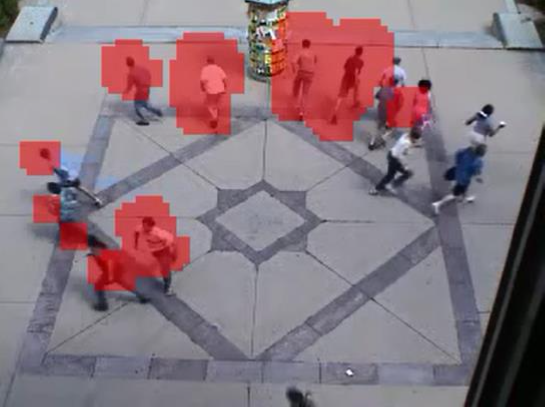
\includegraphics[width=0.7\linewidth]{fig1}
	\caption{人群四散逃离的异常事件(全局异常事件)}
	\label{fig:fig1}
\end{figure}

\begin{table}
    \centering
	\caption{一张表} \label{tab:tab1}
	\begin{tabular}{lrrr} \hline
		年份        & 乡村 & 城市 & 所有   \\ \hline
		1983        & 38.7  & 55.6  & 44.7  \\
		1993–1994   & 50.3  & 66.4  & 54.3  \\
		2004–2005   & 50.2  & 69.3  & 55    \\
		2009–2010   & 51.7  & 71.6  & 57.1  \\ \hline
		\multicolumn{4}{@{}l@{}}{\footnotesize 来源: http://tomheaven.cn}
	\end{tabular}
\end{table}

\begin{figure}
    \centering
	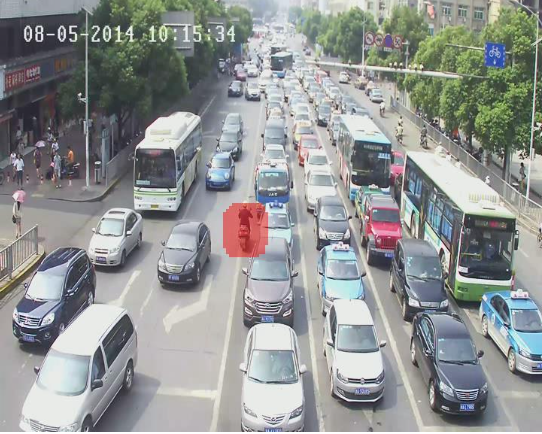
\includegraphics[width=0.7\linewidth]{fig2}
	\captionof{figure}{摩托车违章逆行的异常事件(局部异常事件)} % \caption{} 改为
	\label{fig:fig2}
\end{figure}




\subsubsection{广义异常事件}

本课题认为从分类的角度检测到的是特定类型异常事件\upcite{2-5_2},而从概率的角度检测到的是广义异常事件\upcite{li2000}。例如打架斗殴、人群逃散、交通事故都是根据人们的先验知识确定的异常事件,在绝大多数场景中,只要发生这样的事件,就肯定是异常事件。而广义异常事件与特定类型异常事件相对,是指不能由人们的先验知识预先设定类别,而是由监控视频场景决定的异常事件。发生概率低和与场景相关是广义异常事件的本质特征。

例如图 2的摩托车逆行,只有发生在此场景的城市道路上,才是异常事件。如果发生在了无人烟的乡村土路上并不算是异常。而摩托车是不是逆行,也只有放在此特定的场景中才能判断。

\subsection{研究意义}
    随着视频监控在商场、银行、小区、道路等公共场所的广泛部署\upcite{Cong2011Sparse},监控视频数据大量产生。目前监控视频主要还是用于威慑犯罪和事后调取,但视频智能分析的需要一直存在。近期发生了一些引起公众关注的事件再次体现了监控视频异常检测需求的迫切性。IBM深圳公司的一名女经理在地铁口突发心脏病跌倒,虽然正对着监控,却因为监控无人查看而耽误了抢救时间,最终不幸去世。对于这种紧急情况,仅有八分钟的黄金抢救时间,不能及时发现险情和施救生命就会逝去。
    监控视频的异常检测在安防领域、交通管理、城市管理方面有广阔的应用前景。从监控视频中自动发打架斗殴、交通违章、交通事故、人群聚集等事件具有及时发现事故险情,提前发现安全隐患的作用。例如图 3中的行人违规横穿马路,说明此路段存在交通安全隐患,有必要派出交警或者增设警示标志。如果这种情况持续发生,可以考虑架设人行天桥来引导行人。而这种安全隐患靠人工是很难发现和统计的。

  随着计算能力的不断进步,满足视频智能分析需求的计算成本在不断降低,视频智能分析的技术也在不断进步,为监控视频智能分析的普及准备着技术条件,智能监控的时代正在迫近。异常事件检测,作为视频智能分析的重要一环,能够帮助及早发现安全隐患,对异常事件实时发出警报,对于利用监控视频保障安全、处置险情,有重要作用\upcite{biblatex}。


%%% ++++++++++++++++++++++++++++++++++++++++++++++++++++++++++++++++++++++++++++++++++
